\chapter{System Design\label{sec:tech77}}

\section{System Overview}
The PDU is responsible for transferring energy to subsystems and payloads, which makes him vital and extremely important part of the satellite. 

 According to the Chapter \ref*{cha:chapter3}, main requirement of the PDU is to be able to distribute a power into subsystems and payloads, which is accomplish by having a 23 power lines. Each power line is controlled by load switch, which is enabled by the signal from the microcontroller. Every power line is measured by analog current sensor that amplify its signal to the ADC. The ADC converts analog input into a digital output and communicate to the microcontroller via SPI protocol. Due to GPIO pins limitation of the microcontroller, it was decided to use a shift register to control additional load switches by using an I$^2$C protocol. 
 
 
  Figure \ref{fig: PDU} Illustrates the simple Power Distribution Unit architecture block diagram.\\ \\


 \begin{figure}[h]
 	\centering
 	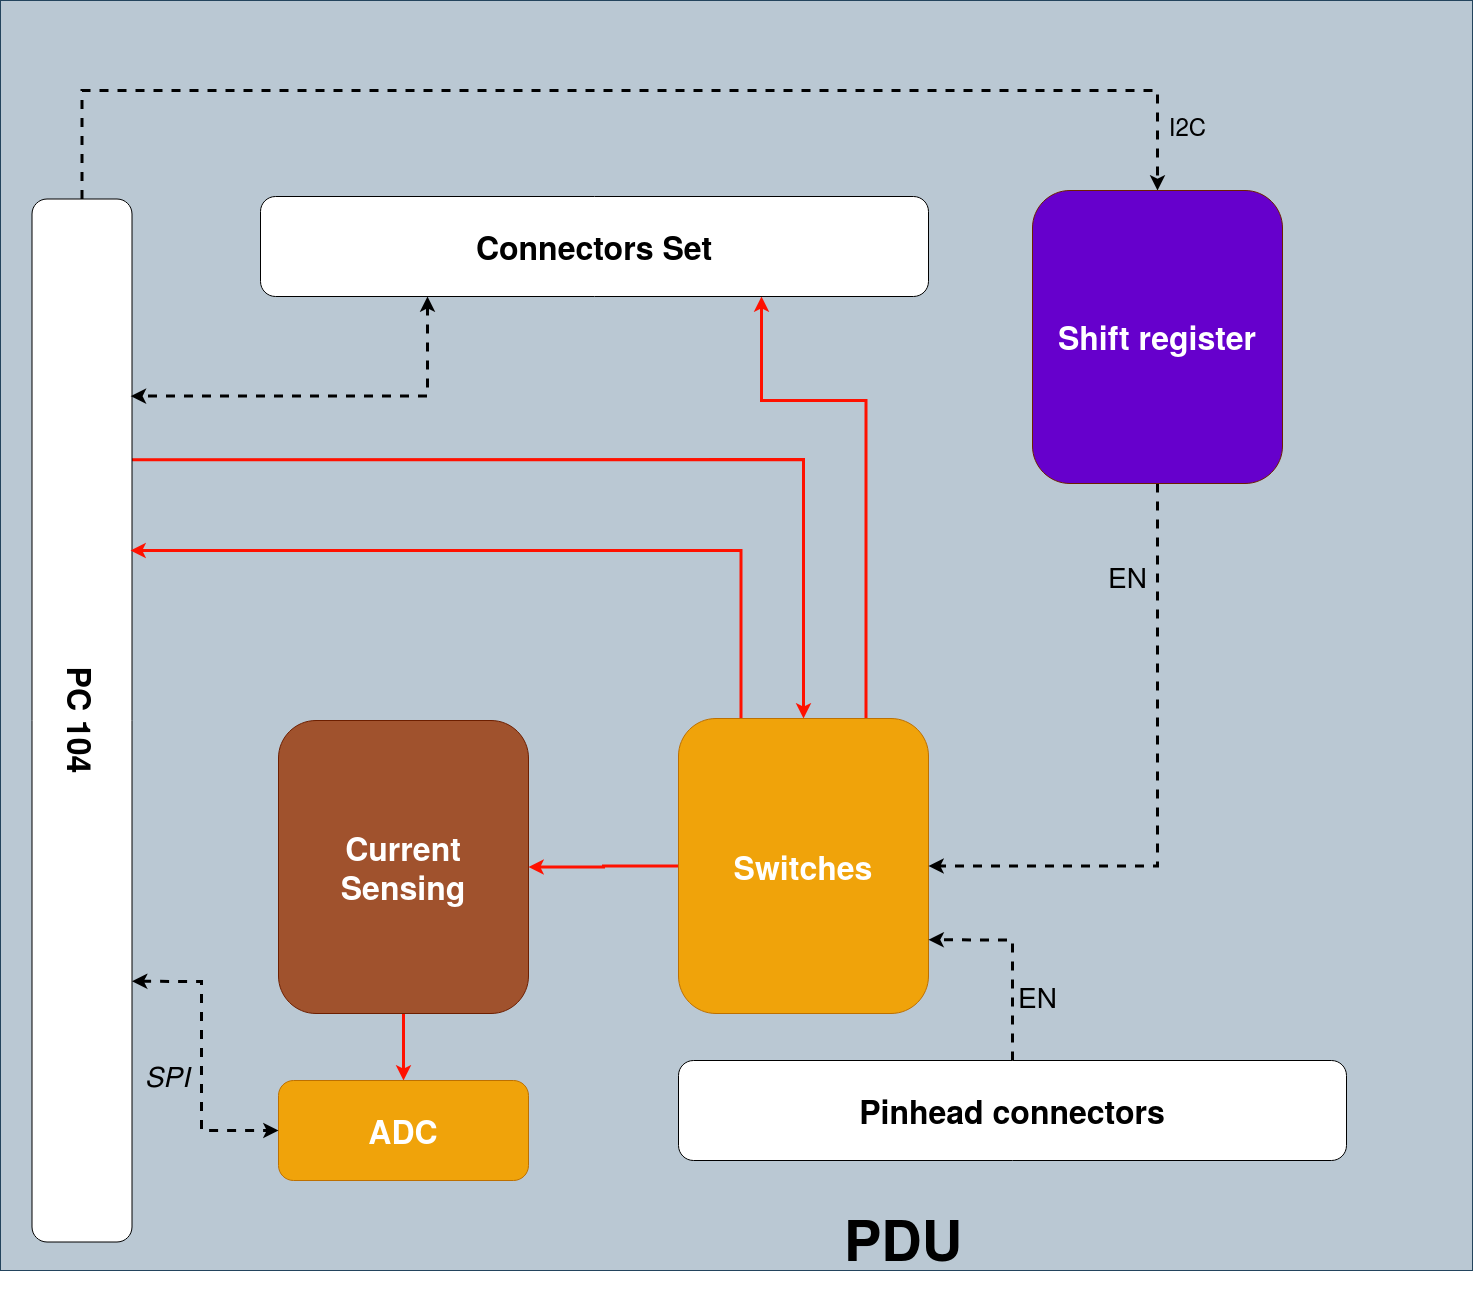
\includegraphics[scale=0.19]{PDU.png}
 	\caption{PDU board}
 	\label{fig: PDU}
 \end{figure} 

\section{Load Switches}
PDU has 23 power load switches which provide commutation of the power lines. In order to fulfill the demanded requirements from Chapter \ref{cha:chapter3}, three types of load switches were chosen: TPS203x, TPS1H200A and FPF2701. 
\captionof{table}{Switches and power lines of the PDU}
\begin{tabular}{p{2cm}p{2cm}p{2cm}p{2cm}p{2cm}p{2cm}} \toprule
	Channel & Switch  & Voltage [V] & Type & Output\\ \midrule
	VCC0 & TPS203x & 3.3, 5 & BUS & PC104\\
	VCC1 & TPS203x & 3.3, 5 & BUS & PC104\\
	VCC2 & TPS203x & 3.3, 5 & BUS & PC104\\
	VCC3 & TPS203x & 3.3, 5 & BUS & PC104\\
	VCC4 & TPS203x & 3.3, 5 & BUS & PC104\\
    VCC5 & TPS203x & 3.3, 5 & BUS & PC104\\
    VCC6 & TPS1H200A & 5, Vbat & BUS & PC104\\
    VCC7 & TPS1H200A & 5, Vbat & BUS & PC104\\
    VCC8 & TPS203x & 3.3, 5 & Payload & Side con.\\
    VCC9 & TPS203x & 3.3, 5 & Payload & Side con.\\
    VCC10 & TPS1H200A & 5, Vbat & Payload & Side con.\\
    VCC11 & TPS1H200A & 5, Vbat & Payload & Side con.\\
    VCC12 & TPS1H200A & 5, Vbat & Payload & Side con.\\
    VCC13 & TPS1H200A & 5, Vbat & Payload & Side con.\\
    VCC14 & TPS1H200A & 5, Vbat & Payload & Side con.\\
    VCC15 & TPS1H200A & 5, Vbat & Payload & Side con.\\
    VCC16 & TPS203x & 3.3, 5 & Payload & Side con.\\
    VCC17 & TPS203x & 3.3, 5 & Payload & Side con.\\
    VCC18 & TPS1H200A & 5, Vbat & Payload & Side con.\\
    VCC19 & TPS203x & 3.3, 5 & Payload & Side con.\\
    COM0 & FPF2701 & 7.4 & BUS & PC104\\
    COM1 & FPF2701 & 7.4 & BUS & PC104\\
    HISP & TPS1H200A & 5, Vbat & BUS & PC104\\ \\
	\bottomrule
	
\end{tabular}\\ \\ \\ \\

Every switch has the ability to determine over current($\overline{OC}$)of its power line and provide a signal to the microcontroller. Then, the microcontroller which will open all switches for a determined time and close them again in order to prevent latch up of the power lines. All pins of the $ \overline {OC} $ PDU switches are connected star-type to one pin of the P1 connector, which prevents system destruction due to a single node failure.

In addition, each switch of the PDU board can adjust the required current limit on the line by configuring the current limit resistors or changing the type of chips that fit to the IC's footprint.    
  \\ \\
\subsection{TPS203x }
The TPS203x switch has an operating voltage of 2.7 V to 5.5 V, which can be used for both 3.3 V power line and 5 V power line. TPS203x is a easy to use 8 pin micro chip. Fig. \ref{fig: PDU332} illustrates the pinout of the load switch TPS203x.

\begin{figure}[h]
	\centering
	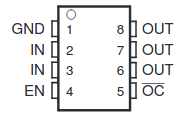
\includegraphics[scale=0.6]{tps203x.png}
	\caption{TPS203x \cite{26}}
	\label{fig: PDU332}
\end{figure} 

TPS203x has  two power input pins 2,3 and three output pins 6, 7, 8. Load switch control, provided by a microcomtroller, communicates with TPS203x via EN pin 4. TPS203x also has a required ability to provide an over current signal by pin number 5 $\overline{OC}$. \cite{26} When the output load exceeds the current, $\overline{OC}$ getting LOW and the switch limits the output current to a safe level by switching into a constant current mode. TPS203x has 4 different types of chips: TPS2030, TPS2031, TPS2032, TPS2033, TPS2034. All of these chips have a different current threshold. Current limit of five TPS203x types shown on the table \ref{Tab:curr}.\\

\captionof{table}{Types of TPS203x and their curret limits\cite{26}}
\begin{tabular}{p{4cm}p{5cm}p{4cm}} \toprule
	Switch type & Recommended max continuous  current [A] & Current Limit [A]\\ \midrule
	TPS2030 & 0.2 & 0.3\\
	TPS2031 & 0.6 & 0.9\\
	TPS2032 & 1 & 1.5\\
	TPS2033 & 1.5 & 2.2 \\
	TPS2034 & 2 & 3 \\
	
	\bottomrule
	
\end{tabular}\\ \\ \\ \\
\label{Tab:curr}

Each type of TPS203x switch has been selected to meet the requirements of the power line according to Table \ref{Tab:curr}. Switch TPS2030 is used on the lines: VCC0, VCC1, VCC3, VCC4, VCC5, VCC9 and VCC19  where supplied voltage is not beyond the tolerance of 5.5V and load current does not exceed the limit of 0.2A. Switch TPS2031 is used on the line VCC17 for the LORA payload where supplied voltage is not beyond the tolerance of 5.5V and load current does not exceed the limit of 0.6A. Switch TPS2032 is used on the line VCC8 for the AURA payload where supplied voltage is not beyond the tolerance of 5.5V and load current does not exceed the limit of 1A. Switch TPS2033 is used on the line VCC2 for the ADCS where supplied voltage is not beyond the tolerance of 5.5V and load current does not exceed the limit of 1.5A. Switch TPS2034 is used on the line VCC16 for the antenna release mechanism where supplied voltage is not beyond the tolerance of 5.5V and load current does not exceed the limit of 3A. \\

Figure \ref{fig: vcc0} illustrates the switch TPS2030 on the power line VCC0, which is used to supply power to the OBC.

\begin{figure}[h]
	\centering
	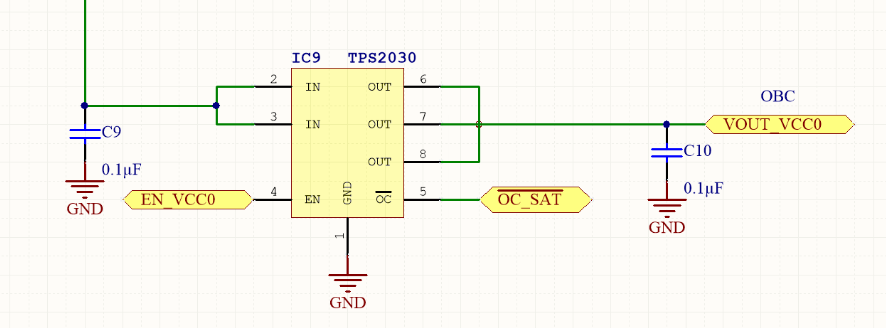
\includegraphics[scale=0.4]{tps203x_.png}
	\caption{TPS2030 on the VCC0 channel}
	\label{fig: vcc0}
\end{figure} 

From the Figure \ref{fig: vcc0}, two bypass capacitors C9 and C10 used to filter the signal and to improve the immunity of the device to short-circuit transients.   Additionally, 10k pull up resistor connected to the $\overline{OC}$ (10K pull up resistor shown in Appendix C). \\ \\

\subsection{FPF2701}

FPF2701 has an operating voltage 2.8 to 36V and 0.4 to 2A adjustable current limit. FPF2701 has an SO8 footprint package. In addition, FPF27001 was used on previous 3U satellite missions.\\

\begin{figure}[h]
	\centering
	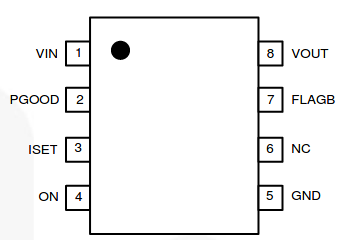
\includegraphics[scale=0.3]{fpf2701.png}
	\caption{FPF2701 \cite{27}}
	\label{fig: fpf27}
\end{figure} 

FPF2701 is the 8 pin load switch which is used for the UHF power line commutation. FPF2701 completely fulfill requirements TL13, TL14 from Chapter \ref{cha:chapter3} regarding the UHF power supply. It can handle the required voltage of 7.4V and adjust the current to needed 690mA. The most important feature of FPF2701 load switch is the inverted enable input(active LOW).\\

Pin 1 is a power input pin which can handle the voltage between 2.8 and 36V. Pin 3 ISET used to adjust the current limit of the load switch. \cite{27} "The  current  limit  ensures  that  the  current  through  the switch  doesn't  exceed  a  maximum  value  while  not limiting  at  less  than  a  minimum  value.  The current-limit level    is    adjustable    through    an    external    resistor connected between the ISET pin and GND. " The formula \ref{eq:fpf} shows the calculation of the resistor value for intended current limit value.

\begin{equation}\label{eq:fpf}
R_{set}(k\Omega) = \frac{277.5}{I_{lim}(A)}
\end{equation}

For the Descartes mission, the current limit $I_{lim}$ was defined to 2A to prevent an inrush current pike influence, which was achieved by setting the resistor to 140K.

Pin 4 of the FPF2701 is an inverted enable pin, which was required according to FR7 the Chapter \ref{cha:chapter3}. FLAGB (pin 7) is the open drain pin that provides a signal to notify the microcontroller when the adjusted current of the ISET pin is exceeded. FLAGB provide a 3.3V output to the microcontroller. In case the current limit is exceeded, the control logic of the chip sends signal to the inner MOSFET that connect ground with the pin. All fault pins such as $\overline{OC}$, FLAGB  are connected to the one connector pin with a star type, which prevent the system from collapsing in case of the failure of one node.

\begin{figure}[h]
	\centering
	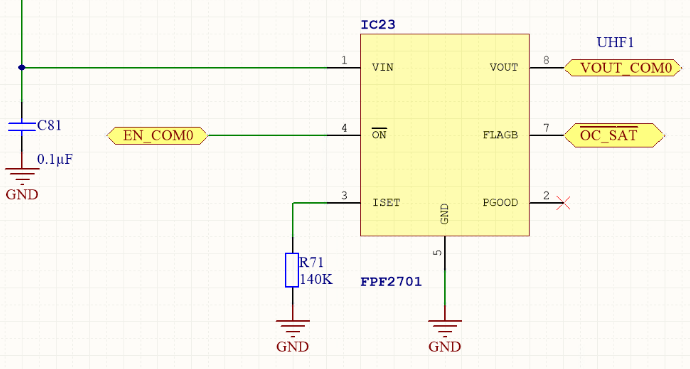
\includegraphics[scale=0.3]{fpf2701_pic.png}
	\caption{FPF2701 on the COM0 power line}
	\label{fig: fpf27_schema}
\end{figure} 

\subsection{TPS1H200A}

TPS1H200A \cite{28} has an operating voltage 3.4V to 40V and an adjustable current up to 6A. TPS1H200A has a 8-pin HVSSOP footprint package. Descartes Mission and PDU design, according to top level requirements, TL1 and TL3, require a switch capable of switching the voltage of 5V and 7.4V which is inside the tolerance of the TPS1H200A chip. Second reason of choosing TPS1H200A chip has the ability to configure the current limit by external adjustment resister  which fulfill requirement FR5. Third reason is the ability to determine over-current on the line and notify the microcontroller. Moreover, the chip was used for previous satellite missions.\\

Descartes Mission require eight Vbat power lines, where Vbat equals 7.4V. However, PDU design consists of ten power lines which used TPS1H200A switch. One of the reasons for this - opportunity to work on 5V and handle a big loads up to 6A. \\ 

Switch TPS1H200A is used for on lines VCC10, VCC11, VCC12, VCC13, VCC14, VCC15 which used to supply power to DeCor payloads. Also switch TPS1H200A is used on empty lines VCC6, VCC7 and VCC18. Finally, TPS1H200A used on HISP power line, which provide power to Hispico transceiver. 

TPS1H200A has 8 pins and thermal pad which is connected to GND. Pin 1 is enable pin which activates the power transmission of the switch. Signal to the switch comes from the GPIO pin of microcontroller. Pin 2 enables diagnostic function of the TPS1H200A chip. While diagnostic function is activated TPS1H200A is able to set up current limit, adjust delay and provide a current limit signal to a microcontroller. Pin 3 provide an output signal to microcontroller when current limit was surpassed. Pin 4 allow to adjust current limit. Current limit threshold can be set by placing an external resistor. Equation \ref{eq: res} shows the resistor value calculation.

\begin{equation}\label{eq: res}
R = \frac{0.8 \times 2500}{I}
\end{equation}


Pin 5 is a DELAY pin which configure the behavior of the chip while over current. When current limit is reached, TPS1H200A supports 3 modes: holding, latch-off and auto retry. For most of the cases TPS1H200A is configured as a latch-off. \cite{28} "When hitting a current limit,the output current holds at the setting current,but latches off after a preset DELAY time ($t_{dl1}$+ $t_{dl2}$). $t_{dl1}$ is the default delay time,and $t_{dl2}$ is a capacitor-configurable delay time." To adjust TPS1H200A as a latch-off external capacitor has to be placed. 

\begin{figure}[h]
	\centering
	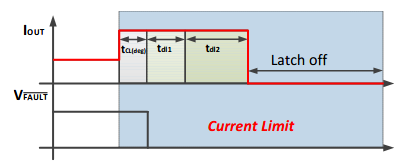
\includegraphics[scale=0.5]{tpscl.png}
	\caption{Latch-off mode\cite{28}}
	\label{fig: tpscl}
\end{figure} 

The time $t_{dl2}$ can be configured by external capacitor by equation \ref{eq: t2}.  \\

\begin{equation} \label{eq: t2}
C_{delay} = \frac{4.5\mu A \times t_{dl2}}{1.45V} 
\end{equation}



 HISP power line, which is needed to supply power to S-band transceiver Hispico, required 5V and load of 1.5A, during the first 0.001s of inclusion Inrush current of the Hispico may reach 4A. The typical inrush current distribution is shown in Figure \ref{fig: hisp_inr}.

\begin{figure}[h]
	\centering
	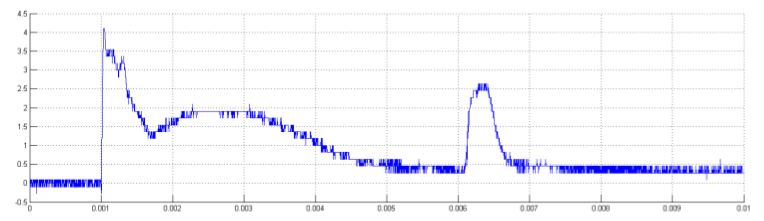
\includegraphics[scale=0.5]{hisp_diag.png}
	\caption{Typical inrush current at startup (0.001 s) in A over time in s}
	\label{fig: hisp_inr}
\end{figure} 

To prevent a critical voltage drop while inrush current, two capacitors with value of 22µF in parallel were placed at output of the load switch. This is illustrated on the figure \ref{fig: hispico}. The value of capacitors was calculated by using formula \ref{eq:3}.

For the TPS1H200A on the HISP channel CL pin is adjusted to 2A and DELAY pin is configured as holding mode. In holding mode \cite{28}"when hitting a current limit,the output current holds at the setting current." This combination was made in order to prevent switch from shutting down while 4A inrush current during the inclusion of Hispico S-band transceiver and keep the threshold at 2A for the required 1.5A load of s-band transceiver. 
 


\begin{figure}[h]
	\centering
	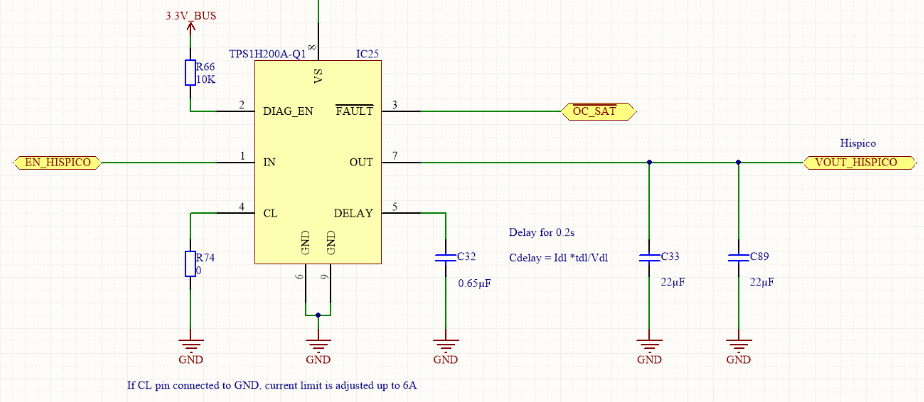
\includegraphics[scale=0.5]{Hispy.png}
	\caption{TPS1H200A on the HISP power line}
	\label{fig: hispico}
\end{figure}



 
\section{Shift Register}\label{shiftty}

Due to the lack of free GPIO pins on the microcontroller, EPS can only provide 17 GPIO channels for PDU. Based on this, it was decided to include a shift register in the design of PDU. PDU in it's design has 5 empty power lines VCC4, VCC5, VCC6, VCC7, VCC18 which are not going to be used for Descartes Mission. All this power lines are enabled via shift register as well as VCC19 which is responsible for triggering the power line, that supplies power to the thermo-sensors. The design idea of having empty power channels and thermo-sensors channel on the shift register, is to include less important power lines under shift register control, thereby exclude the risk of the pin control via additional device. 


 MAX7328 is a two wire  serial-interfaced peripherals with eight I/O ports. MAX7328 has 16 pin SO wide footprint package. \cite{29} MAX7328 is general-purpose port expanders operating from a 2.5V to 5.5V supply that provide eight open-drain output ports with a 20mA sink capability. In addition, integrated pull up resistors are used for the I$^2$C line, which are not shown on the Fig. \ref{fig: sr1}.       MAX7328 has a 3 address inputs A0, A1 and A2. Those address inputs can be configured by soldering the external zero ohm resistors to the appropriate input pins.  


\begin{figure}[h]
	\centering
	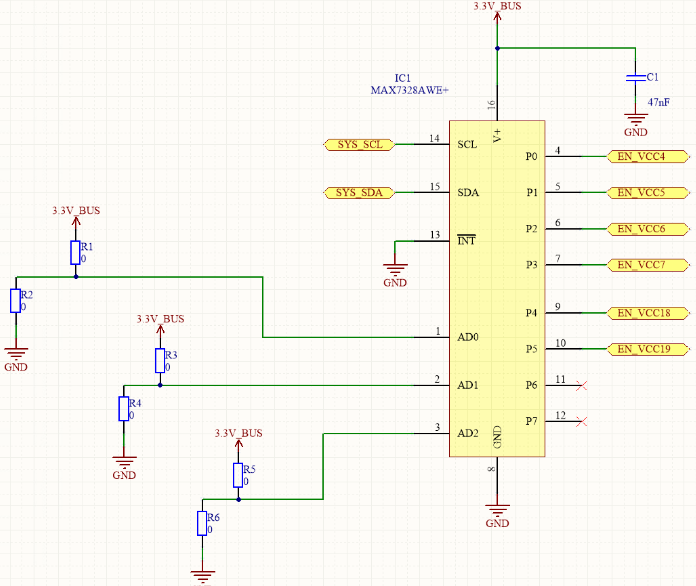
\includegraphics[scale=0.3]{sr.png}
	\caption{ Schematics of the shift register MAX7328}
	\label{fig: sr1}
\end{figure}

The MAX7328 shift register has easy operation principle. The control of the shift register implemented via I$^2$C protocol. The microcontroller must communicate with the slave device (MAX7328) by sending the address of the slave device to the I$^2$C bus, which must be accompanied by a confirmation bit, then port data can be sent to enable or disable the port. The operation principle of MAX7328 is shown on the Fig. \ref{fig: sr_op1}. 
\newpage
\begin{figure}[h]
	\centering
	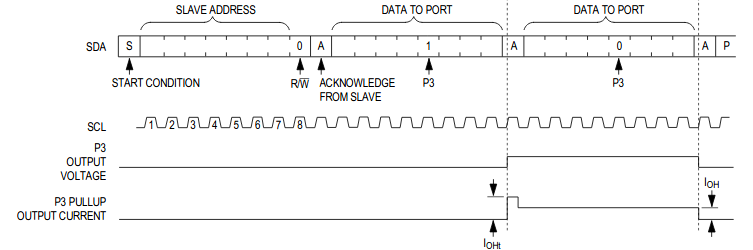
\includegraphics[scale=0.5]{sr_op.png}
	\caption{ MAX7328 operation principle\cite{29}}
	\label{fig: sr_op1}
\end{figure}
 
\section{Current Measurement and Conversion}

Due to the fact that PDU requires to have 23 current sensors for each power line, it was decided to use 23 analog current sensors in combination with an ADC. The main reason for this choice is to keep the flight heritage which was used for previous missions. Second reason is a relatively huge amount of sensors. Current sensors that give an output directly to I$^2$C or SPI have a limited amount of slaves which make them unsuitable to use for the current application.\\

For the Descartes Mission used MAX4372T current sensor. MAX4372 is a current-sense amplifier which offer a gain of 20. MAX4372T operates on 3.3V and draws 30 µA. MAX4372 has a compact SOT23-5 package with 5 pins. Figure \ref{fig: max4372t_inside} illustrates the functionality of max4372T current sensor.

 \begin{figure}[h]
 	\centering
 	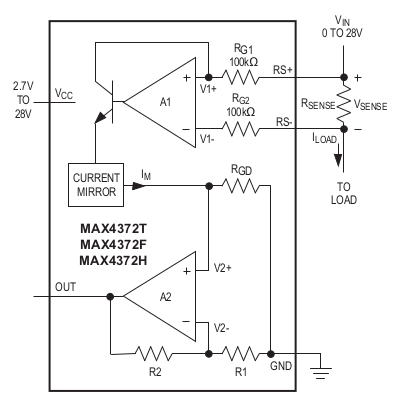
\includegraphics[scale=0.4]{max4372inside.png}
 	\caption{MAX4372T \cite{24}}
 	\label{fig: max4372t_inside}
 \end{figure} 

\cite{23}"Current flows through the sense resistor, generating a
sense voltage  Since
A1’s inverting input is high impedance, the voltage on
the negative terminal equals V IN - V SENSE . A1 forces its
positive terminal to match its negative terminal; therefore,
the voltage across $R_{G1}\times (V_{IN} - V_{1}-)$ equals $V_{SENSE}$ . This
creates a current to flow through $R_{G1}$ equal to $V_{SENSE}$ /
$R_{G1}$ . The transistor and current mirror amplify the current
by a factor of $\beta$. This makes the current flowing out of the
current mirror equal to: 

 \begin{equation}
I_{M} = \frac{\beta \times V_{sense}}{R_{G1}}
 \end{equation}
 A2’s positive terminal presents high impedance, so this
 current flows through $R_{GD}$ , with the following result:
  \begin{equation}
V_{2+} = \frac{R_{GD} \times \beta \times V_{sense}}{R_{G1}}
  \end{equation}
  R1 and R2 set the closed-loop gain for A2, which ampli-
  fies $V_{2+}$, yielding:
  \begin{equation}
  V_{out} = \frac{R_{GD} \times \beta \times V_{sense}}{R_{G1} \times (1+\frac{R2}{R1})	 }
  \end{equation}
The gain of the device equals:
  \begin{equation}
  GAIN =\frac{V_{out}}{V_{sense}} = \frac{R_{GD} \times \beta (1+\frac{R2}{R1})}{R_{G1}}
  \end{equation}
  
  MAX4372 has 3 types of current sensors, for a MAX4372T type, amplification factor equal 20.
  
  Considering different current lines and the fact that ADC has a limited tolerance of the analog input, $R_{sense}$ have to be chosen correctly according to the requirements. According to the datasheet of the ADC(MAX1231) the analog input has to be between $ -0.3V$ and $(V_{DD} + 0.3V)$ where $V_{DD}$ equals 3.3V.
  
  The value of $R_{sense}$ could be calculated with a formula:
    \begin{equation}
    R_{sense} = \frac{V_{out}}{GAIN \times I}
    \end{equation}
  
  Where:\\
  I is a current on the power line\\
  V$_{out}$ is an output voltage\\ 
 
 The Tab. \ref{Tab:res} provide a calculated values of the shunt resistors according to the current recuirements of the power lines. V$_{out}$ = 0.5V was chosen as a reference output voltage for the shunt resistor selection. This value is in the tolerance and allows to choose shunt resistor with lower value to decrease the voltage drop.
  \newpage
  
  \captionof{table}{Shunt resistor choosing}
   \begin{tabular}{p{3cm}p{3cm}p{2cm}p{2cm}p{3cm}} \toprule
   	Power channel & Load & I$_{max}$ [mA] & V$_{out}$ [V] & R$_{sense}$ [Ohm]\\ \midrule
   VCC0 & OBC & 140 & 0.5 & 0.1\\
   VCC1 & OBC PH & 140 & 0.5 & 0.1\\
   VCC2 & ADCS & 460 & 0.5 & 0.05\\
   VCC3 & ADCS log & 0.06 & 0.5 & 0.5\\
   VCC4 & OBC 5V & 90 & 0.5 & 0.1\\
   VCC5 & OBC 5V & 90 & 0.5 & 0.1\\
   VCC6 & empty & empty & empty & empty\\
   VCC7 & empty & empty & empty & empty\\
   VCC8 & AURA & 600 & 0.5 & 0.05\\
   VCC9 & AMUR & 40 & 0.5 & 0.5\\
   VCC10 & DeCor11 & 40 & 0.5 & 0.5\\
   VCC11 & DeCor12 & 200 & 0.5 & 0.1\\ 
   VCC12 & DeCor21 & 40 & 0.5 & 0.5\\ 
   VCC13 & DeCor22 & 200 & 0.5 & 0.1\\ 
   VCC14 & DeCor31 & 40 & 0.5 & 0.5\\ 
   VCC15 & DeCor32 & 200 & 0.5 & 0.1\\ 
   VCC16 & ARM & 2000 & 0.5 & 0.01\\
   VCC17 & LORA & 200 &  0.5 & 0.1\\
   VCC18 & empty & empty & empty & empty\\
   VCC19 & Term. sens. & 10 & 0.5 & 2.5\\
   COM0 & UHF1 & 690 & 0.5 & 0.05\\
   COM1 & UHF2 & 690 & 0.5 & 0.05\\
   	HISP & HISPICO & 1500 & 0.5& 0.01\\ 
    \bottomrule
   	
   \end{tabular}\\ \\ \\ \\
  \label{Tab:res}
 Another important aspect to consider is the resistance of the power line. The resistance of the power line should be as low as possible to avoid voltage drop in the presence of high current. In the system design stage, voltage drop can be avoided by providing a low shunt resistor value. In accordance with current requirements, the HISP and VCC16 power channels must provide $ \ geq $ 1500mA, with a resistance of 1Ohm the system will have a voltage drop of $ \ geq $ 1.5V, which will significantly affect the functionality of the output connected device.
 For this reason resistor values for HISPICO and ARM(antenna release mechanism) were chosen with minimal resistance.\\ \\ 
 
 6U satellite contain 23 analog outputs from the current sensors which have to be converted into a digital signals. To fulfill this requirement, two analog-to-digital converters MAX1231 are used. MAX1231 has already been used for previous 3U mission, in order to preserve the heritage of the flight, it was decided to keep this component for the 6U satellite.
 
  \cite{25}MAX1231 is a serial 12 bit  analog-to-digital converter with an internal reference and maximum sampling rate of 300ksps. MAX1231 has a 24 pin configuration with 15 available analog inputs and. The device operates at 3.3 V and contains 10 MHz SPI protocol for communication.
  
   \begin{figure}[h]
   	\centering
   	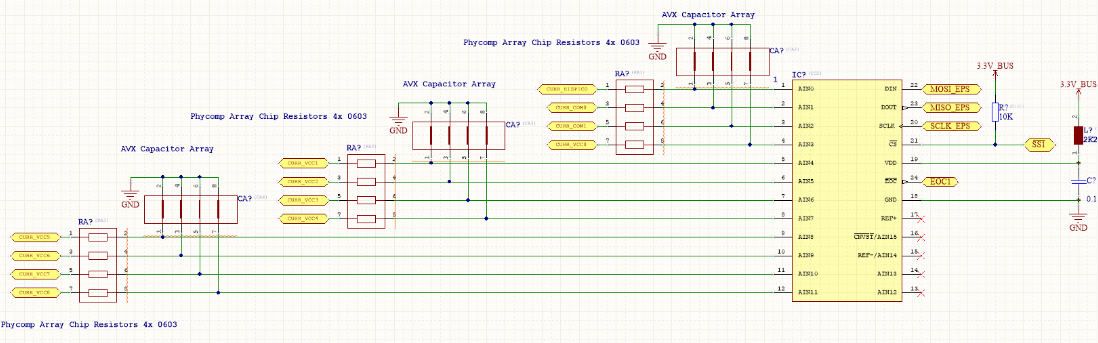
\includegraphics[scale=0.4]{ADC.png}
   	\caption{MAX1231 for Descartes application}
   	\label{fig: adc}
   \end{figure} 
 
  Figure \ref{fig: adc} illustrates the MAX1231 for the Descartes application. This figure shows external connections of the ADC chip. Pins 1 to 12 used for the analog inputs. Each analog input has a 1k resistor, which is used to protect the ADC and prevent high current input from the sensor. In addition, decoupling capacitors with a capacity of 0.01µF are located in parallel, which are used to filter the input signal. Pins 22, 23, 20 and 21 are used for the SPI communication where pin 21 is a slave select. Pin 24 is the $\overline{EOC}$ End of Conversion output pin used to notify the microcontroller about the end of conversion. Pin 19 is a power supply pin for the ADC chip, supplied with a 3.3V. To minimize the noise effect, the VDD input bypassed the 0.1 µF capacitor to GND. In addition, 2.2K ferrit chip connected in series with the supply to improve power-supply filtering. 
 
  \begin{figure}[h]
  	\centering
  	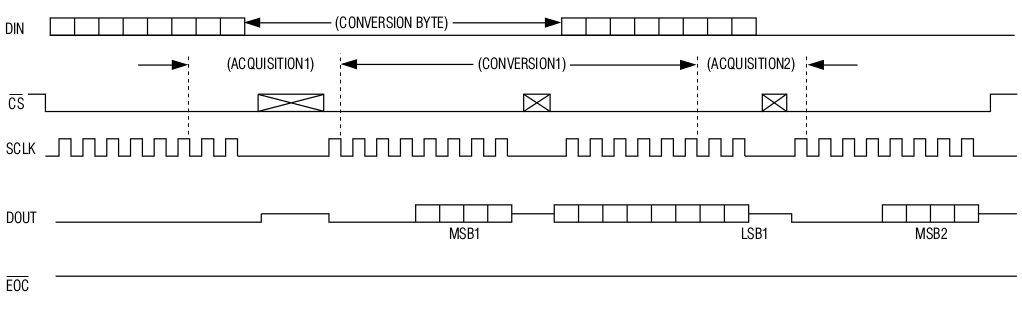
\includegraphics[scale=0.4]{ADC_clock.png}
  	\caption{Clock mode of the MAX1231 \cite{25}}
  	\label{fig: adc}
  \end{figure} 
 
 The MAX1231 has 4 different clock modes. However, the Descartes Mission uses an external clock mode from the microcontroller.  To begin communication with the MAX1231, chip select pin has to be latched up in order to define the slave. Then microcontroller sends a conversion register address with the channel information. After the Register address transmission, slave will send 12 bytes of data separated in two bytes. First receiving byte contain first 4 empty bits which has to be ignored and following 4 bits which are MSB. The second following byte contain the left 8 bits. After the second byte has been sent to the microcontroller, the $ \ overline {EOC} $ pin gets HIGH to notify the microcontroller that the conversion is complete, and the $ \ overline {CS} $ pin becomes LOW.
 
 \section{Isolators}
 
The principle of operation of electrical isolators is the partial separation of electricity from the system for safety reasons during maintenance work. PDU include two payload connectors that carry I$^2$C and SPI signals from the payloads. Due to the functional requirement FR4 from chapter \ref{eq:3} every payload I$^2$C and SPI nodes shall have the isolation. For that reason was made a decision to include well known from the previous missions two types of isolators:\\ \\

$\bullet$ ADUM1250\\
$\bullet$ MAX1485\\ \\

ADUM1250 \cite{30} is a "hot swappable digital isolators with nonlatching, bidirectional communication channels that are compatible with I2C interfaces. This eliminates the need for splitting I2C signals into separate transmit and receive signals for use with standalone optocouplers."

 \begin{figure}[h]
 	\centering
 	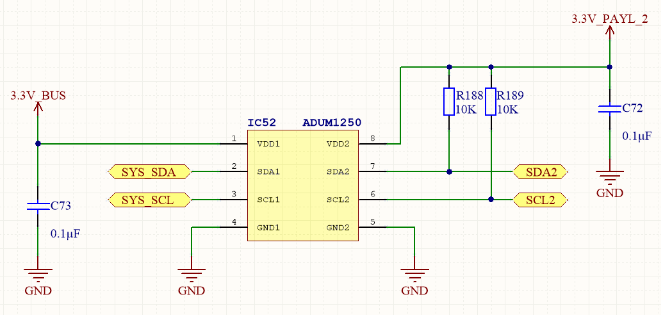
\includegraphics[scale=0.4]{ADUM1250.png}
 	\caption{ADUM1250 isolating main I$^2$C from the payload 2 }
 	\label{fig: adum}
 \end{figure} 

\cite{31} The MAX14850 is a six-channel digital isolator that provides low-cost digital signal transfer between circuits with different power supplies. The MAX14850 provides low power consumption and stable operation at high temperatures. The MAX14850 can be used to insulate SPI buses, I2C buses, RS-232, RS-485 / RS-422 buses, and general purpose insulation.

\begin{figure}[h]
	\centering
	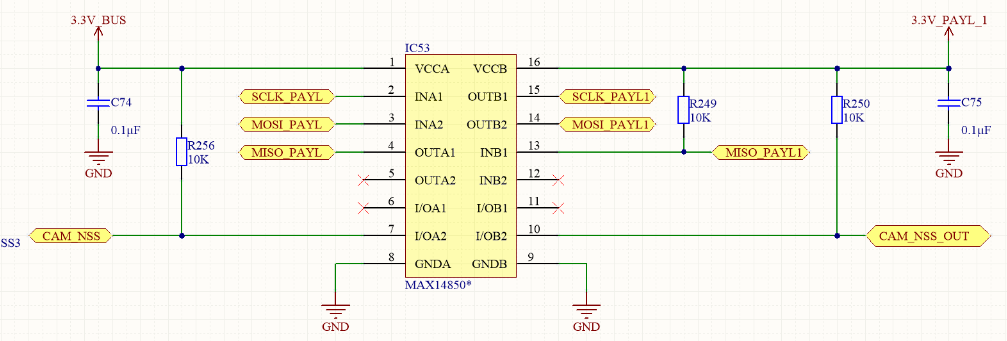
\includegraphics[scale=0.4]{max14850.png}
	\caption{MAX14850}
	\label{fig: adum}
\end{figure} 

\section{Connectors Design}

Power Distribution Unit has 12 connectors on it's design. \\

$\bullet$ eight payload connectors\\
$\bullet$ two EPS connectors\\
$\bullet$ one EGSE connector\\
$\bullet$ one PC104 connector\\

PC104 is a main connector which used to bridge main pcb boards such as PPU, PDU, OBC, OBC-PH, UHF module and Hispico transceiver.
EGSE connector used to program the EPS and OBC microcontrollers, that located on the PPU and OBC boards by using JTAG pins.

EPS connectors P1 and P2 were added into design due to the lack of free pins on the PC104 connector. These connectors provide a signal and power junction between PPU and PDU. EPS connectors provide a enable signals from the EPS microcontroller directly to the PDU via P2 connector and bus power lines 3.3V and 5V via P1 connector.

  \begin{figure}[h]
  	\centering
  	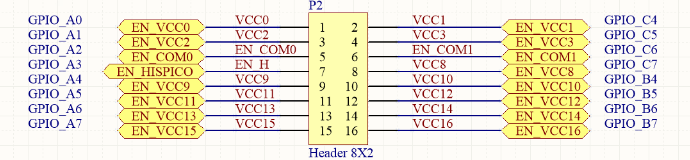
\includegraphics[scale=0.4]{EPSCON.png}
  	\caption{EPS connector P2}
  	\label{fig: EPSCON}
  \end{figure} 

Payload connectors have a primary function to transfer the signal and power to the payload. Eight payload connectors divided into 8-pin connectors and 9-pin connectors. 8-pin connectors designed to carry payloads that require UART and CAN protocols. 9th pin required for the payloads that transfer I$^2$C and SPI protocols in order to give a power feedback into the ADUM1250 or MAX14850 isolators.  

Two payload connectors K10 and K11 were made to include a possible opportunity to handle a payload that require a I$^2$C or SPI protocols.
The connection design of connector K10 is illustrated on the figure \ref{fig: iso1}. To adjust the signal input between I$^2$C and SPI simple zero ohm resistors are used.

\begin{figure}[h]
	\centering
	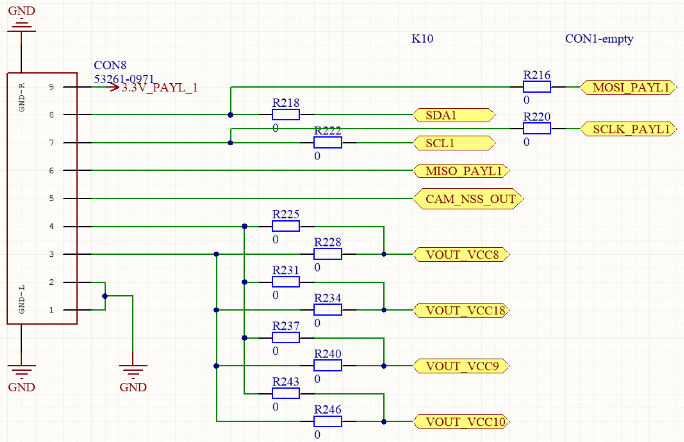
\includegraphics[scale=0.4]{iso1.png}
	\caption{Payload connector K10}
	\label{fig: iso1}
\end{figure} 
 
PDU designed in the way that all payload connectors have an opportunity to be supplied from different sources and with different voltages. The reason for this is the functional requirement FR1 in the chapter \ref{eq:3}. This design allow PDU to be compatible with every payload requirement. Every payload connector has ability to transfer at least 3.3V, 5V and 7.4V to the payload. This requirement was accomplished with zero ohm  resistors that adjust the input of the power supply to the payload connector.

All connectors and their pin descriptions shown in the Annex. 

 
  
  